Dette afsnit kommer til at handle om hvordan man kan beskrive dette projekts problemområde, som er en husholdnings administration af pligter og børne økonomi, i form af klasser og hændelser. Klasser er overordnede repræsentationer af objekter, som for eksempel en enkel Pligt eller et Barn. Hændelser er de begivenheder og ændringer, som klasserne kan forårsage eller blive påvirket af. Klasser kan normalt blive beskrevet som et navneord, for eksempel en Forælder eller en Pligt, mens hændelser kan blive beskrevet som udsagnsord, for eksempel en Forælder som opretter en ny Pligt, og et Barn som efterfølgende optager denne Pligt. Klasser og hændelser for dette problemområde er blevet sat op i en hændelsestabel, som kan blive set på tabel \ref{Haendelstabel}. En plads som har et plustegn betyder, at den tilsvarende kun forekommer en gang pr. klasse instans, og et gangetegn betyder at det kan forekomme flere gange.

\begin{table}[H]
	\centering
	\begin{tabular}{| l | l | l | l | l | l | l | l | l |}
	\hline
	& \textbf{Pligt Opretning} & \textbf{Optagelse} & 
	\textbf{Anmodning Opretning} & \textbf{Behandling} & 
	\textbf{Færdiggørelse} & \textbf{Se Ledige} & 
	\textbf{Hæve} & \textbf{Se Statistik} \\ \hline
	\textbf{Forælder} & * &  &  & * & * & * & * & * \\ \hline
	\textbf{Pligt} & + & * &  &  & + &  &  &  \\ \hline
	\textbf{Barn} &   & * & * &  & * & * & * & * \\ \hline
	\textbf{Model} & * &  &  &  & * &  &  &  \\ \hline
	\textbf{Anmodning} &  &  & + & + &  &  &  &  \\ \hline
	\end{tabular}
	\caption{Hændelsestabel.}
	\label{Haendelstabel}
\end{table}

Tabellen giver et overordnet overblik til sammenhængen mellem klasser og hændelser, og være beskrivende for de mere væsentlige dele af problemområdet. En Anmodning er i denne sammenhæng en besked et barn sender til sin Forælder om, at det har fuldført en af sine tilskrevne pligter, og ønsker denne behandlet.

Klasserne kan herefter blive sat op i klasse diagram, som viser de indbyrdes sammenhænge mellem klasserne i problemområdet. Se figur \ref{KlasseDiagram}. Klassehierarkier bliver vist indkapslet i kasser, samt pile fra underklasser til superklasser. Rene streger viser associering, som Model og Forælder, hvor lommepenge modellen går ind og påvirker på hvad forældrene gør i forhold til pligter og udbetalinger. En klasse som tilhører en anden klasse bliver vist med en pil, ligesom for klassehierarkiet, men med en rombe i stedet for en pil. Ligeledes angiver tallene mængden af hver klasse til en anden klasse. For eksempel så er en pligt altid kun forbundet til den Forælder som lavede den, mens en Forælder sagtens kan lave adskillige pligter.

\begin{figure}[H]
\centering
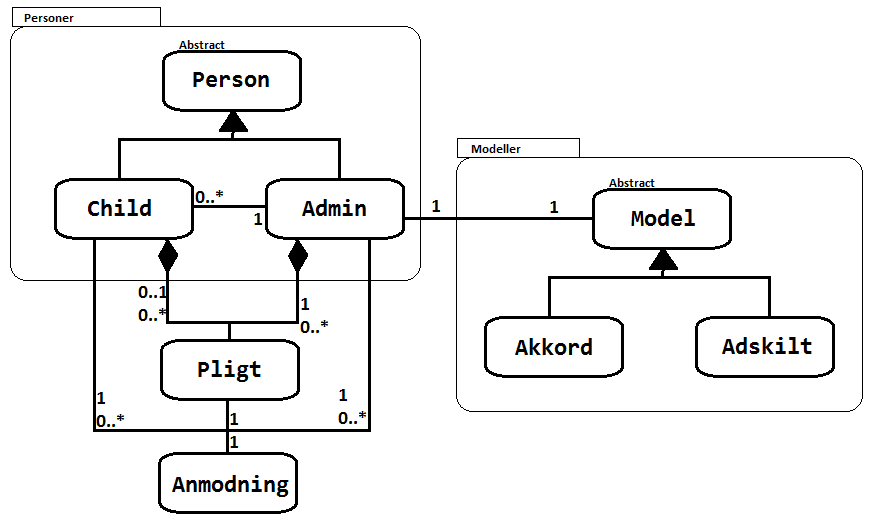
\includegraphics[width=0.8\textwidth]{Billeder/KlasseDiagram.png}
\caption{KlasseDiagram.}
\label{KlasseDiagram}
\end{figure}

Ud fra den foregående hændelsestabel samt klassediagram kan man beskrive klasser mere detaljeret ved hjælp af hændelsesforløb diagrammer. Hændelsesforløb går ind på hver klasse, og viser, hvordan et objekt af en klasse opstår i problemområdet og systemet, og hvad der sker med det indtil det ’dør’. Pile viser hændelser som hver klasse kan udføre, eller som kan blive udført på dem. Hændelser kan også forårsage, at et objekt skifter tilstand, som bliver vist med tilstands bokse. Hændelser kan også føre tilbage til den samme tilstand boks, som betyder hændelses kan blive udført adskillige gange. Det følgende viser fire hændelsesforløb for dette problemområde. Metode hændelsesforløbet er blevet udeladt, som sagt fordi den går ind og påvirker andre områder i systemet, og vil derfor ikke gøre andet end at være aktiv, indtil den bliver udskiftet.

\begin{figure}[htb]
\centering
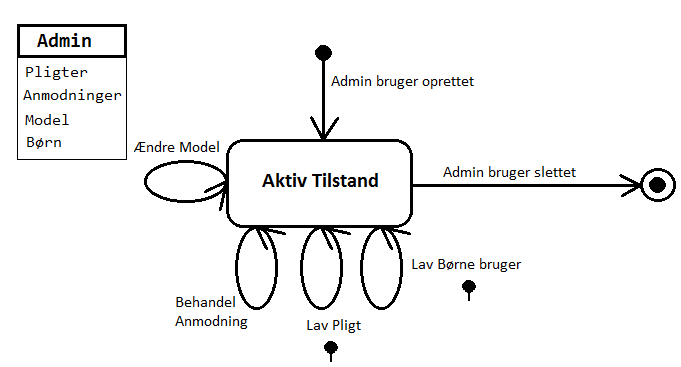
\includegraphics[width=0.8\textwidth]{Billeder/ForaelderForloeb.png}
\caption{Forælder Hændelsesforløb.}
\label{ForaelderHaendelsesforloeb}
\end{figure}

\begin{figure}[htb]
\centering
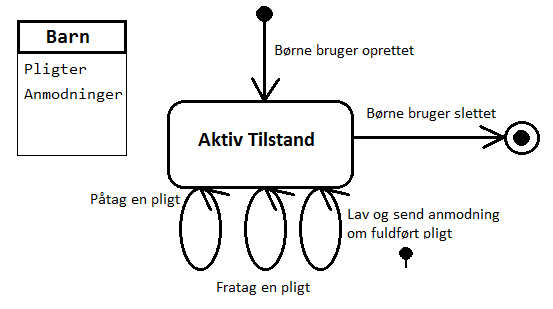
\includegraphics[width=0.8\textwidth]{Billeder/BoernForloeb.png}
\caption{Barn Hændelsesforløb.}
\label{BarnHaendelsesforloeb}
\end{figure}

\begin{figure}[htb]
\centering
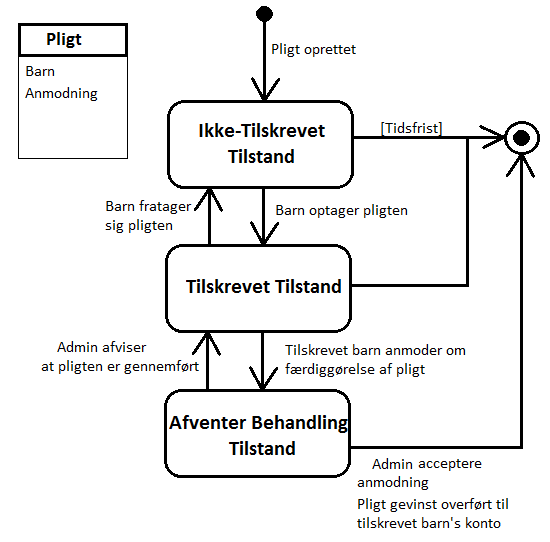
\includegraphics[width=0.8\textwidth]{Billeder/PligtForloeb.png}
\caption{Pligt Hændelsesforløb.}
\label{PligtHaendelsesforloeb}
\end{figure}

\begin{figure}[htb]
\centering
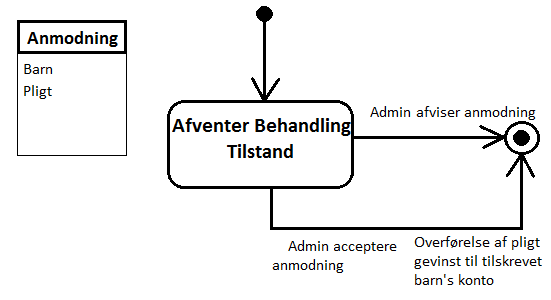
\includegraphics[width=0.8\textwidth]{Billeder/AnmodningForloeb.png}
\caption{Anmodning Hændelsesforløb.}
\label{AnmodningHaendelsesforloeb}
\end{figure}